\cotefile{78}
\scanpage{89}
On retrouve encore une fois que \deleted{\unsure{Cela|le}} la donnée ici coïncide avec ce que nous avions appelé (dans le cas des \unsure{``polygônes|polygônes|n-polygônes} réguliers avec $n$ premier à la car. $p$) ``l'invariant numérique'' dudit. Cependant ici le cas \unsure{d'|de'}une racine double
\[
\unsure{\zeta|\rho}=\zeta' \quad \text{i.e.}\quad \zeta^{2}=1 \quad \text{i.e.}\quad \zeta=\pm1 \tag*{(35)}
\]
n'est pas exclu, il correspond au cas
\[
\alpha=\pm2 \qquad \text{ou encore}\quad \Delta(\alpha)=0 \tag*{(36)}
\]
($\alpha=2$ correspond à $\zeta=1$, $\alpha=-2$ à $\zeta=-1$, les deux cas venant se confondre \unsure{sss|ssi} $p=2$).

\unsure{Celà|Cela} tient compte précisément des 2 seules valeurs de $\zeta$ que ns avions été obligés d'exclure, pour définir nos repr. géom. can. $\varphi^\zeta=(\varphi_{\unsure{s|5|0}}^\zeta,\varphi_{\unsure{a|0|o|1}}^\zeta)$ de $\Pi_\infty$ ! [Le cas $\zeta=1$, $\alpha=2$ est également distingué \deleted{\unsure{en}} comme le seul cas où il n'y ait pas de centre à distance finie .... ]
% archive sheet number: 88
\scanpage{90}
\deleted{5. Étude des cas \unsure{ex}}
\uline{NB} On retrouve, pour $\alpha\ne\pm2$ i.e. $\unsure{\zeta|\rho}\ne\pm1$, les représentations $\varphi^\zeta$ de $\Pi_\infty$, \inserted{du moins si $\zeta\in k$.} Donc \uline{les seuls cas nouveaux} (sur $k$ alg. clos) sont précisément les cas $\alpha=\pm2$ (i.e. $\zeta=\pm1$) qu'on avait été amené précédemment à exclure. Nous allons les étudier séparément au § suivant.
Notons dès à présent que, même si on décidait (à tort !) de ne pas s'intéresser à ces deux cas, considérés comme trop ``exotiques'', les développements en coordonnées canoniques restent intéressants, car a) ils sont valables pour tt corps, et $\unsure{=|\overline{m}}$ tout anneau, de base $k$, et \deleted{b) ils} \inserted{pas \unsure{seult}} pour $k$ alg. clos, et b) ils permettent de suivre la variation de \deleted{$\unsure{\Pi|\varphi}$} $\varphi(\alpha)$ en termes du paramètre $\unsure{\alpha,|\alpha_s}$ intrinsèque \deleted{\unsure{a}}\unsure{.|-}
% archive sheet number: 89
\scanpage{91}
5) \uline{Étude par cas}.

I) $\Delta(\alpha)\ne0$ \quad i.e. $\alpha\ne\pm2$ \quad (``cas ordinaire'')

Étendant au besoin le corps de base $k$ en $k(\unsure{\zeta|\rho})=k(\zeta')$, et rapportant maintenant $E$ au nouveau syst. de coordonnées de centre $o$, ayant comme axes les droites propres de $u$ $D_\zeta$ et $D_{\zeta'}$, et pour lesquels $s_0$ est de coordonnées $(1,1)$, on trouve par un argument déjà fait le cas-type $\Pi_\zeta$ (où $\zeta$ n'est pas \unsure{néc$^{t}$} une racine de 1).
Il y a une fonction quadratique (\unsure{p.r. au centre|par son centre} $o$) invariante, canonique à un scalaire multiplicatif près, qu'on peut normaliser en exigeant que sa valeur en les sommets de $\Pi_\zeta$ soit égale à 1.. L'image \deleted{$\Pi_\zeta$} \inserted{de la représentation $\Pi_\zeta$} est un polygône géométrique, dont le nb de \unsure{côté|cté|côtés}, égal à l'ordre de $\zeta$, est (\deleted{s'il} \inserted{quand il} est fini) premier à la caractéristique.

\deleted{II) \uline{$\alpha=-2$}} \deleted{On supposera ici $\alpha\ne2$ (i.e. $p\ne2$),}
\[
\begin{aligned}
&\deleted{\unsure{\sigma|v|r}_0(x,y)=(1-x-2y,y)}\\
&\deleted{u_0(x,y)=(1-y-2x,x)}\\
&\deleted{u_0^2(x,y)=(1-x-2(1-y-2x),1-y-2x)}\\
&\qquad\deleted{=-1+3}
\end{aligned}
\]
\deleted{de sorte que l'on a encore \unsure{l'existence|existence} et le centre $o$.}
% archive sheet number: 90
\scanpage{92}
II Considérons \unsure{le|les} cas $\alpha=\pm2$, donc $\unsure{\zeta|\rho}=\pm1$

On aura pour la partie homogène \inserted{$u_0$} de $u$
\[
\begin{aligned}
u_0\deleted{\unsure{\varepsilon|k}}&=\varepsilon(\mathrm{id}+v_0) &\varepsilon&=\pm1,\quad v_0^2=0\\
\text{\unsure{sc.|i.e.}}\qquad v_0&=\varepsilon u_0-\mathrm{id}
\end{aligned}
\]
De façon explicite
\[
\begin{aligned}
u(x,y)&=(1-\deleted{\unsure{x}}y+2\varepsilon\deleted{\unsure{y}}x,x)\\
u_0(x,y)&=(-y+2\varepsilon x,x)\\
\unsure{v|u}_0(x,y)&=(x-\varepsilon y,\varepsilon(x-\varepsilon y))=(x-\varepsilon y)(1,\varepsilon)\\
&&=\deleted{\unsure{\varepsilon|k}}a'(z)a
\end{aligned}
\]
où \deleted{$a'$ est la \unsure{for|f}} $a'\in\check V,\ a\in V$
\[
\left\{\begin{aligned}
a'(x,y)&=x-\varepsilon y\\
a&=(1,\varepsilon)
\end{aligned}\right.
\]
% archive sheet number: 91
\scanpage{93}
\[
\begin{aligned}
u^2&=(1-x+\alpha(1-y+\alpha x),1-y+\alpha x)\\
&=((1+\alpha)+(\alpha^2-1)x-\alpha y,1+\underset{\deleted{\unsure{2}}}{\alpha x}-y)\\
&\deleted{=(\unsure{-|+|{}}1+3x+2y,1\unsure{.}}\\
&\unsure{,}\;3+3x-3y,1+2x-y
\end{aligned}
\]
\[
\begin{aligned} x&=y\\2x&=\alpha y\qquad\alpha\ne2\end{aligned}
\]
\[
\left\{\begin{aligned}
\sigma_1(\deleted{\unsure{x}}X,\deleted{\unsure{y}}Y)&=(Y,X)\\
\sigma_0(X,Y)&=(-X+\alpha Y,Y)\\
u(X,Y)&=(-Y+\alpha X,X)
\end{aligned}\right.
\]
\[
\begin{aligned}
\alpha&=-2 &\deleted{u(X,Y)=}\quad\unsure{.}\\
&&u=-(1+v),\quad v=-\mathrm{id}-u\\
&&\hspace{9em}=\\
u(X,Y)&=(-Y\deleted{\unsure{+}}-2X,X)\\
v(X,Y)&=(\deleted{\unsure{-}}\underbrace{X+{}}Y,-(X+Y)) & v^2=0
\end{aligned}
\]
\figure{\begin{tikzpicture}[x=1cm,y=1cm]
\draw (-1.15,-.04) -- (0,0) -- (1.7,.08);
\draw (-.07,-.73) -- (0,0) -- (0,1.12);
\draw (-1.28,1.10) -- (0,0) -- (.91,-.94);
\draw (1.07,-1.09) -- (1.49,-1.52);
\fill (0,0) circle (.055);
\node[left] at (-1.30,1.10) {$\deleted{\unsure{t|D}}$};
\end{tikzpicture}}
\[
\deleted{v(\unsure{x|z}}\qquad
\left\{\begin{aligned} u^2&=1+2v=\left(\begin{matrix}1&\\0&1\end{matrix}\right.\\ &\phantom{1}\end{aligned}\right.
\]
\[
\left\{\begin{aligned}\sigma_1(x,y)&=(y,x)\\\sigma_0(x,y)&\end{aligned}\right.
\qquad\begin{aligned}
u_V&=\underset{\substack{\parallel\\\pm1}}{\varepsilon}(1+v)\\
u&\qquad\unsure{.}
\end{aligned}
\]
\[
\begin{aligned}
u(X,Y)&=(-Y+2\varepsilon X,X)=\varepsilon(\\
u_V&=\varepsilon(\mathrm{id}+v) &v&=\varepsilon u_V-\mathrm{id}\\
v(X,Y)&=\big(\overset{X'}{\overline{X-\varepsilon Y}},\overset{Y'}{\overline{\varepsilon\underline{(X-\varepsilon Y)}}}\big)
& &=(X-\varepsilon Y).(1,\varepsilon)\\
&&&X=\varepsilon Y
\end{aligned}
\]
\[
\begin{aligned}
&\deleted{=\quad X'\unsure{-|=}\varepsilon Y'}\\
&\deleted{\varepsilon X'}\qquad\deleted{=X}\\
&\deleted{\unsure{X-Y}\;X-\unsure{Y}\quad X\unsure{+}}\qquad\deleted{\unsure{X-}}\\
&\deleted{X-\varepsilon^2X\qquad X'-\varepsilon Y'=0}
\end{aligned}
\]
\[
\left(\begin{aligned}
&(X+Y,-(X+Y)\\
&(X-Y,+X-Y)
\end{aligned}\right.
\]
% archive sheet number: 92
\scanpage{94}
% letterhead
CEREMADE\\
CENTRE DE RECHERCHE DE MATHEMATIQUES DE LA DECISION\\
ERA \quad CNRS \quad N° 249\\
Université Paris IX Dauphine\\
Paris\unsure{\textasciidieresis|\textquotedbl} le 10 novembre 1977\\
\handwritten{A. GROTHENDIECK}\\

Mon Cher Collègue,\\

Je me permets de vous rappeler ma lettre du 26 octobre 1977 concernant le refus des autorités soviétiques de laisser A. D. IOFFE rejoindre son poste de professeur associé sur contingent national.

J'ai depuis lors appris qu'il avait protesté auprè\`{s} de M. GROMIYKO, Ministre des Affaires Etrangères de l'Union Soviétique, en démontrant que la raison invoquée pour justifier de ce refus était fausse.

J'ai aussi appris le nom d'une personne responsable de ce refus : il s'agit de

V. Semenitin, Académicien\\
Académie des Sciences de l'Union Soviétique\\
Leninsky Prospect 14\\
Moscou\\

Je vous serai reconnaissant si vous pouviez lui écrire pour lui demander d'utiliser son influence pour que IOFFE soit autorisé à venir en France avec sa famille (définitivement, si cela est possible).

Ces lettres peuvent faire l'objet de pétitions signées par les membres de votre UER.

En vous remerciant, bien amicalement.\\
\handwritten{\unsure{Jean|J. A.}}\\
Jean-Pierre AUBIN\\

P.S. Si cela vous est possible, pouvez-vous m'addreser une copie de vos lettres que vous avez écrites afin que je puisse centraliser les informations.

% letterhead
Place du Maréchal De Lattre de Tassigny \quad 75775 PARIS Cedex 16 - Téléphone \quad 553.50.20
% archive sheet number: 93
\scanpage{95}
I) $\alpha\ne\pm2$ \quad (valeurs propres distinctes de $u_V$, \unsure{exste|existe} centre)

\deleted{Sur l'extension \unsure{$k_\zeta$|finie} \unsure{extension} $k'$ de $k$}
Si $k$ contient les racines $\unsure{\zeta|\rho},\zeta'=\zeta^{-1}$ de l'équ aux valeurs propres, alors \unsure{can.|cas|on est} isom. à \deleted{$\Pi_\zeta$} $\varphi_{\unsure{\zeta}}$ \dots{} Ordre de $u_V$ est égal à celui de $u_E$ \unsure{de même|du moins|ou encore} à celui de $\zeta$.
\deleted{II) $\alpha=-2$, $\alpha\ne2$}
\deleted{II) Cas $\alpha=\unsure{\pm|-}1$ i.e. valeurs propres confondues} \deleted{\unsure{II)} Cas $\alpha={}$} \deleted{II) Cas $\alpha=-2$, $\alpha\ne2$ il y a}
\[
\deleted{u=\begin{pmatrix}\unsure{1{-}2|-2}&-1&1\\1&0&0\\0&0&1\end{pmatrix}}
\]
\[
\begin{aligned}
\text{II)}\quad\alpha&=-2\qquad \zeta=\zeta'=-1&
\deleted{u_V^{\unsure{2}}=\mathrm{id}}\quad u_V^2&=\text{transvection}\\
&&&\text{d'ordre }p\\
&&u_V&\ \text{d'ordre }2p\\
&&u_E&\ \text{d'ordre }2p\text{ si }p\ne2\\
&&&(\text{car }\exists\text{ centre})
\end{aligned}
\]
$\overline{\mathrm M}$ conclusion si $p=2$. En effet, on a alors $\alpha=-2=0$, or le cas $\alpha=0$ est celui du \uline{carré} ($\zeta^2=-1$ \unsure{§|!}\dots)
\[
\begin{aligned}
\deleted{\sigma_{\unsure{0}}(x,y}\quad u(x,y)&=(1-y,x)\\
u^2(x,y)&=(1-x,1-y)\\
u^4(x,y)&=(x,y)\qquad\cdots
\end{aligned}
\]
Si $p\ne2$, \inserted{i.e. $\alpha\ne2$,} on trouve, en posant
\[
\left\{\begin{aligned}X&=x\unsure{-|+}\frac{1}{2-\alpha}\\Y&=y\unsure{-|+}\frac{1}{\unsure{2|7}-\alpha}\end{aligned}\right.
\]
\[
\begin{aligned}
\left\{\begin{aligned}\sigma_0(x,y)&=(-X+\alpha Y,Y)\\\sigma_1(X,Y)&=(Y,X)\\u(X,Y)&=(-Y+\alpha X,X)=-(\mathrm{id}+a'\otimes a)(X,Y)\end{aligned}\right.\\
a'(X,Y)=X+Y\qquad a=(1,-1)
\end{aligned}
\]
% archive sheet number: 94
\scanpage{96}
\figure{\begin{tikzpicture}[x=.78cm,y=.78cm,>=stealth]
\draw (0,-.07) -- (0,1.62) node[left] {$1$};
\fill (0,1.62) circle (.035);
\draw (0,0) -- (1.97,-.01) node[right] {$1$};
\draw (-1.95,2.47) -- (1.87,-1.98);
\draw[->] (-.73,.83) -- (-1.56,1.76);
\draw (-.76,2.04) -- (2.53,-1.48);
\draw (-.74,.83) -- (-1.17,.42) -- (-.46,-.39);
\draw[->,very thick] (-.46,-.43) -- (1.92,1.52);
\draw[->,very thick] (0,0) -- (1.91,-1.99) node[below right] {$a$};
\draw (1.84,-.39) -- (1.77,-1.77);
\fill (0,0) circle (.045) (-.46,-.43) circle (.085) (.51,.46) circle (.085) (-1.17,.42) circle (.075);
\draw (2.53,-1.48) circle (.05);
\node at (-.85,2.13) {$\unsure{o|0}$};
\node[right] at (1.92,1.57) {$\unsure{a|x}$};
\node[right] at (.55,.42) {$s_0$};
\node[below] at (-.58,-.50) {$-s_0$};
\node[left] at (-1.36,.12) {$-s'_0$};
\node at (-1.81,-.34) {$\parallel$};
\node[left] at (-1.23,-.88) {$-(s_0+\tfrac12a)$};
\end{tikzpicture}}
\[
s_0:\ \deleted{\unsure{\zeta|x|X}}\left(\frac1{2-\alpha},\frac1{2-\alpha}\right)=\left(\frac14,\frac14\right)
\]
\[
\begin{aligned}
u&=-(\mathrm{id}+v_0)\\
u^2&=\mathrm{id}+2v_0\\
\left\{\begin{aligned}u^{2n}&=\mathrm{id}+2n v_0\\u^{2n+1}&=-(\mathrm{id}+(2n+1)v_0)\end{aligned}\right.
\end{aligned}
\]
\[
s_{2n}=s_0+2n\underbrace{v_0(s_0)}_{(\frac12,-\frac12)}
=s_0+n\underbrace{(1,-1)}_a=s_0+na
\]
\[
s_{2n+1}=-(s_0+(2n+1)v_0(s_0))=-s_0\unsure{-|+}(n+\tfrac12)a
=(-s_0\unsure{-|+}\tfrac12a)\unsure{-|+}na
\]
\begin{center}\rule{1.7cm}{.35pt}\\[-1.5ex]\rule{1.2cm}{.35pt}\end{center}
III) \uline{$\alpha=+2$} \quad (Pas de centre) \quad $\unsure{\zeta|\rho}=\zeta'=+1$
\[
\begin{aligned}
\deleted{u_V\ \text{d'ordre }p}\qquad u_V&=\mathrm{id}+v_0\qquad v_0=a'\otimes a\ne0,\quad \unsure{u|v}_0^2=0\\
u_V&\ \text{d'ordre }p
\end{aligned}
\]
Je dis que $u_E$ d'ordre $p$, sauf si $p=2$ (déjà traité, où on trouve $2p=4$)
\deleted{$u_E$} Du point de vue de l'enveloppe vectorielle
\[
\begin{aligned}
u_E&=\mathrm{id}+w &w^3&=0\\
u_E^p&=\mathrm{id}+\deleted{\unsure{p}}w^p \quad\deleted{\unsure{pour|si}\ p\unsure{>}} &p\ge3&\quad\text{on gagne}
\end{aligned}
\]
\deleted{$p=2$ on trouve} [pour $p=2$, on trouve $u_E^2=\mathrm{id}+w^2\ne\mathrm{id}$ \unsure{donc|car} $w^2\ne0$]
% archive sheet number: 95
\scanpage{97}
6) \uline{\unsure{formes|forme} quadratiques \unsure{invariante|invariantes}}.

On s'intéresse aux expressions
\[
\deleted{f}F(x,y)=ax^2+bxy+cy^2+ux+vy+d
\]
polynômiales de degré $\le2$ sur $E$, qui correspondent aux formes quadratiques sur l'enveloppe vectorielle $\unsure{\mathcal E|\mathscr E|\hat E}$ de $E$. On cherche celles qui sont invariantes par $G=\mathrm{Aut}\,\Pi$, i.e. par $\sigma_0,\sigma_1$. Il y a les constantes, donc on est ramené à voir les conditions pour que \deleted{$f$ soit \unsure{inv.}} \inserted{l'expression sans} terme constant
\[
\deleted{f}F(x,y)=ax^2+bxy+cy^2+ux+vy
\]
soit invariante. L'invariance par $\sigma_1$ signifie que $f(x,y)$ est symétrique en $x,y$
\[
\begin{aligned}
a=c,\quad u=v\qquad \text{i.e.}\\
\deleted{f}F(x,y)=a(x^2+y^2)+bxy+u(x-y)
\end{aligned}
\]
et quand on explicite l'invariance par $\sigma_0$, on trouve
\[
\deleted{f}F=a f_{\unsure{\alpha|*}}
\]
\[
\boxed{f_\alpha(x,y)=(x^2-x)+(y^2-y)-\alpha xy}
\]
Les fonctions $f$ \inserted{(pol. de degré $\le\unsure{2|?}$)} nulles sur $S$ invariantes par $G$ sont les multiples \unsure{de|du} $f_\alpha$ ci-dessus.
% margin note written sideways
\margin{NB}
% archive sheet number: 96
\scanpage{98}
Les fonctions $1,\unsure{f_\alpha|f}$ forment une base \inserted{sur $k$} de l'\unsure{ens|esp|ens.} des fonctions pol. de degré $\le2$, inv. par $G$.
% margin note written sideways
\margin{\uline{Conique circonscrite (canonique)} $\unsure{C(f)|C[f]|C(f_\alpha)}$ définie par $f=0$ (\unsure{indépndte|indépendte} de \deleted{\unsure{la}} normalisation). On vérifie que si $\alpha\ne0,1$ (i.e. cas du polyg. régulier à $n\ge5$ côtés) c'est la \uline{seule} conique circonscrite}
Parmi ces fonctions, $f$ est caractérisée par les \deleted{fonctions} conditions

a) $f_\alpha$ nulle sur $S$

b) La ``partie homogène'' \deleted{\unsure{d}}$f_0$ de $f$ satisfait
\[
f_0(s_i-s_{i-1})=1\qquad\forall i
\]
[NB
\[
\begin{aligned}
f_0(\deleted{\unsure{x,y}}X,Y)&=X^2+Y^2-\alpha XY\\
\text{donc}\qquad f_0(1,0)&=1\quad\big]
\end{aligned}
\]
\begin{center}\rule{1.4cm}{.35pt}\end{center}
7/ \deleted{Le discri} \uline{Discriminant de} $f_0$

Le discriminant de $f_0$ est
\[
\delta(f_0)=\deleted{\unsure{\alpha|2}}\;4-\alpha^2=(2-\alpha)(2+\alpha)
\]
qui est nul \unsure{sss|ssi} $\alpha=\pm2$ : la métrique définie par $f_0$ est non dég. sss on a $\alpha\ne\pm2$, i.e. sss on est dans le cas ``ordinaire''. On aura
\[
f_0(X,Y)=(Y-\unsure{\zeta|\rho}X)(Y\unsure{-|+}\zeta'X)
\]
où $\zeta,\zeta'$ sont les solutions de l'équation aux valeurs propres. Les ``\deleted{droites} \inserted{directions} isotropes''
% archive sheet number: 97
\scanpage{99}
(sur une extension $k'$ de $k$ contenant $\unsure{\zeta|\rho},\zeta'$) sont les droites homogènes
\[
\begin{aligned}
&\deleted{\unsure{Y/X|X}=\zeta\ \text{et}}\\
&Y-\zeta X=0\qquad Y-\zeta'X=0
\end{aligned}
\]
qui sont aussi les droites propres sous $u_0$
\[
(\qquad u_0(X,Y)=(-Y+\alpha X,X)
\]
[ce qui correspond au fait que $u_0$ est une \deleted{\unsure{(pour|pour} \illegible{1}} \uline{\unsure{rotation|rotatation}} pour $f_0$, si $f_0$ est non dég. i.e. $\alpha\ne\pm2$]

Dans le cas $\alpha=\pm2$, ces deux directions sont confondues ; \deleted{\unsure{si}} Pour $\alpha=-2$, $\zeta=\zeta'=-1$, on trouve la direction
\[
X\unsure{-|+}Y=0
\]
qui apparaissait déjà comme privilégiée dans l'étude du ``cas II'' \deleted{($\alpha=-2$)}. Pour $\alpha=2$, $\zeta\unsure{=}\zeta'=1$, c'est la direction $X=Y$, \deleted{\unsure{qu}} on va l'examiner plus en détail plus bas.

8) Discriminant \inserted{divisé} de $f$. La matrice de $f$ est
\[
\begin{pmatrix}2&-\alpha&-1\\-\alpha&2&-1\\-1&-1&\deleted{\unsure{2}}0\end{pmatrix}.
\]
son discriminant est égal à
\[
\delta=2\delta'\qquad\delta'=-(\alpha+2)
\]
% archive sheet number: 98
\scanpage{100}
donc $f$ est régulière \unsure{sss|ssi} on a $\alpha\ne-2$. Dans ce cas, la \uline{conique circonscrite} $C(f\deleted{\unsure{\alpha}})$ est non sing.

On notera que c'est le cas en particulier pour $\alpha=+2$, sauf si $k$ est de car. 2. Mais comme $f_0$ est dégénérée, la conique $C(f)$ est une \uline{parabole}.

Dans le cas $\alpha=-2$, on aura
\[
\begin{aligned}
f(x,y)&=(x^2-x)+(y^2-y)+2xy=(x+y)^2-(x+y)\\
&=(x\unsure{+|-}y)(\unsure{\alpha|x}+y-1)=\lambda(x,y)\big[\lambda(x,y)-1\big]
\end{aligned}
\]
i.e. $f$ est le produit de deux fonctions lin affines ayant $\overline{m}$ partie homogène $x+y$. Ainsi $C(f)$ est la réunion des deux droites parallèles\unsure{,} \inserted{(\uline{distinctes})}, d'équations $x+y=0$, $x+y=1$, qui étaient déjà en évidence dans l'étude du cas II (où on avait cependant utilisé les coordonnées
\[
X=x\unsure{-|+}\tfrac14,\quad Y=y-\tfrac14,\quad x+y=X+Y+\tfrac12,
\]
donc les droites précédentes ont comme équations resp.
\[
X+Y=-\tfrac12,\quad X+Y=+\tfrac12\,\unsure{.}\,).
\]
% archive sheet number: 99
\scanpage{101}
9/ \uline{Retour sur le cas} $\alpha=2$, $\alpha\ne-2$ (i.e. $\alpha=2$ en car. $\ne2$).

On a
\[
f(x,y)=(\deleted{\unsure{x^2}}x-y)^2-(x+y)=v^2-w
\]
\[
\text{où}\qquad
\left\{\begin{aligned}v&=x-y\\w&=x+y\end{aligned}\right.
\quad\text{i.e.}\quad
\begin{aligned}x&=\tfrac12(\unsure{v|w}+w)\\y&=\tfrac12(-v+w)\end{aligned}
\]
Le calcul donne pour $u$, défini en coordonnées \unsure{universelles|anciennes} par
\figure{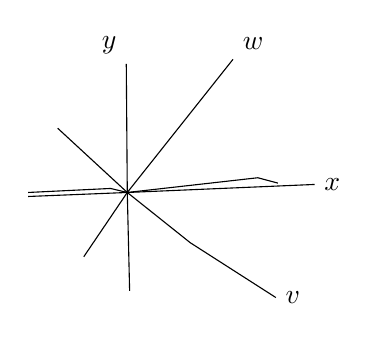
\begin{tikzpicture}[x=.85cm,y=.85cm]
\draw (-1.48,-.06) -- (0,0) -- (2.80,.12) node[right] {$x$};
\draw (-1.48,0) -- (-.25,.06) -- (0,0) -- (1.95,.22) -- (2.25,.14);
\draw (.035,-1.47) -- (0,0) -- (-.015,1.92) node[above left] {$y$};
\draw (-.65,-.96) -- (0,0) -- (1.58,1.99) node[above right] {$w$};
\draw (-1.04,.96) -- (0,0) -- (.94,-.75) -- (2.22,-1.57) node[right] {$v$};
\end{tikzpicture}}
\[
u(x,y)=(1-y+2x,x)
\]
en coordonnées $(v,w)$
\[
U(v,w)=(v+1,1+2v+w)
\]
en particulier, pour des points sur la parabole $C(f)$ d'équation ${\unsure{w|v}}^2-\unsure{v|w}=0$ i.e. $w=v^2$
\[
U(v,v^2)=\deleted{(\unsure{v+1,1+}}\,(v+1,(v+1)^2).
\]
Donc si on paramètre $C(f)$ par la coordonnée $v$, alors $u\mid C(f)$ est décrit par la translation $v\mathrel{\unsure{\mapstochar\relbar\mapstochar|\mapsto}}v+1$ !
% archive sheet number: 100
\scanpage{102}
\uline{Fidélité} d'une réalisation géom. régulière d'un polygône combinatoire.

\uline{Proposition} Soit $\rho=(\rho_{\unsure{S|s}},\rho_{\unsure{A|a}})$ une réalisation géométrique régulière d'un polygône comb. $\underline{\Pi}=(\underline S,\underline A,\underline R)$ sur un corps $k$, \inserted{dans un \deleted{\unsure{espace|p}}plan affine $E$, sur $k$.} Alors l'image $\{\rho_{\underline S}(S)\subset\deleted{\unsure{S}}E,\ \rho_A(A)\subset\mathrm{Dr}(E)\}$ est un polygône géométrique \inserted{$\Pi_0$} régulier dans $E$.
Son groupe d'aut. $G$ est l'image dans $\mathrm{Aff}(E)$ de $\underline G=\mathrm{Aut}(\Pi)$, et $\Pi\unsure{-|\to}\Pi_0$ est \inserted{un hom. de polygônes combinatoires}
a) Toute arête $\rho_A(\underline a)$ ($\underline a\in\underline A$) \unsure{contient} exactement deux sommets. On sait que si $\underline s,\underline{s}'\in\underline S$ sont les 2 sommets incidents à $\underline a$, et $s=\rho_S(\underline s)$, $s'=\rho_S(\underline{s}')$, on a $s\ne s'$.
\deleted{\unsure{Montrons} que $\forall$} \inserted{Soit} $\underline{s}''\in S$, \deleted{tel que} $\rho_S(\underline{s}'')=s''$, \deleted{$a=\mathrm{Dr}(s,s')={}$} $a=\unsure{\psi|\varphi|\rho}_A(\underline a)=\mathrm{Dr}(s,s')$, il faut prouver que si $s''\in a$, on a $s''=s$ ou $s''=s'$. On utilise le fait que $a\cap C$ ne peut contenir que 2 points ($C$ conique circonscrite canonique \unsure{\dots)|\dots}
% archive sheet number: 101
